%----------------------------------------
\subsection{Stencil codes}
\label{sect:stencil}
%----------------------------------------
To numerically solve a set of PDEs, iterative methods (finite difference, finite volume or finite element methods) are frequently used to approximate the solution through a discretized (step by step) phenomena. Thus, the continuous time and space domains are discretized so that a set of numerical computations are iteratively (time discretization) applied onto a mesh (space discretization). In other words, in a mesh-based numerical simulation, the PDEs are transformed to a set of numerical computations applied at each time step on all elements of the discretized space domain (the mesh). Among those numerical computations is found a set of numerical schemes, also called \textit{stencil computations}~\cite{spaaTangCKLL11}. 

\begin{figure}[!h]\begin{center}
  \resizebox{9cm}{!}{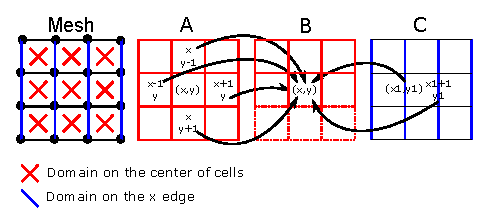
\includegraphics{./images/stencil.pdf}}
  \caption{Example of a stencil computation.}
  \label{fig:ex}
\end{center}\end{figure}

In other words, in a stencil computation the quantity written can be computed using the same quantity at a previous time iteration at $x$ and at $N(x)$. And, any other quantity can also be used in the computation at $x$ and $N(x)$.

%----------------------------------------
\subsection{Multi-stencil programs}
\label{sect:multistencil}
%----------------------------------------
A real case numerical simulation is most of the time composed of a set of numerical schemes (stencils computations), with one or more stencil shape (neighboorhood shape), and onto one or more data. Moreover, a numerical simulation also performs additionnal auxiliary computations which do not involve neighborhood, called local computations. In this paper we target this kind of complex simulations with more than one stencil computation and also additionnal auxiliary computations, that we call \emph{multi-stencil programs}. The work presented produces a general parallelization structure of the overall simulation, while most stencil solutions produce optimized codes for a single stencil code~\cite{citeulike12258902, spaaTangCKLL11, Giles2011}. As it will be detailed in the related work, this work is complementary to most stencil compilers and implicit parallelism languages.

\begin{mydef}
A \textit{stencil computation} is defined as a quadruplet $s(R,w,\text{exp},\mathcal{N})$,
\end{mydef}
where $R$ is the set of data read by the computation, $w$ is the data written by the computation, \textit{exp} is the numerical expression to compute $w$, and $\mathcal{N}$ is a neighborhood shape of the stencil computation.

\begin{mydef}
A local computation is a triplet $l(R,w,\text{exp})$, where $exp$ does not involve a neighborhood function $\mathcal{N}$.
\end{mydef}

A multi-stencil program in this work is defined as a sextuplet
\begin{equation*} 
\mathcal{MSP}(T,\mathcal{M},\mathcal{D}_m,\mathcal{D}_c,\Delta,\Gamma)
\end{equation*}

%----------------------------------------
\subsection{Parallelization techniques}
\label{sect:parallel}
%----------------------------------------
Three parallelization techniques are used in this paper and are described in this section, the data parallelism, the task parallelism, and the hybrid data and task parallelism.

\paragraph{data parallelism} explain data decomposition and distribution, with a single program to apply on each processor

\paragraph{task parallelism} explain task dag

\paragraph{hybrid parallelism} explain the combination


%----------------------------------------
\subsection{Component models}
%----------------------------------------
Component model is an interesting domain of software engineering~\cite{Szyperski:2002:CSB:515228} which improves code re-use, scalability and maintainability of applications~\cite{Szyperski:2002:CSB:515228,bigot:inria-00388508}. Moreover, component models bring a separation of concerns in the application by a clear division of functionnalities in different components. In addition to this, recent work on component models have shown a simultaneous answer to performance, maintainability and portability of applications~\cite{l2c}, which makes this domain an interesting solution to bring maintainability and portability in HPC programming.

Component-based software engineering~\cite{Szyperski:2002:CSB:515228} extends the concept of class by specifying in its interfaces not only the services it offers, or public methods, but also all its possible interactions with outer world, including the services it requires. As a result, each component is an independant entity composed of a set of services its provides, and a set of services it requires (and uses). 

A \emph{port} is an entity embbedded in the component which makes possible an \emph{assembly} of components. An assembly of components (of instanciated components) is a way to actually connect components together and to produce a complete application, as a set of components and their interactions. A provided service inside a component is associated to a \emph{provide} port, while a required service is associated to a \emph{use} port. It is also possible to group more than one required service into a single port, as a list, called a \emph{use-multiple} port. As illustrated in Figures~\ref{fig:ports}, a provide port will be represented by a white circle, a use port by a black circle and a use-multiple port by a black circle with a white $m$ in it.

\begin{figure}[h!]
\begin{center}
\begin{tikzpicture}[shorten >=1pt, node distance=2cm, on grid, auto]
   \node[component] (C) at (0,0) {$Comp_0$};
   \node[provide] (p) at (-1.5,0) {};
   \node[use] (u) at (1.5,0) {};
   \node[use] (um) at (0,1) {$m$};
   \node[provide,right=of u] (p1) {};
   \node[component,right=of p1] (C1) {$Comp_1$};
 
  \path[-]
    (p) edge node {} (C)
    (C) edge node {} (u)
    	edge node {} (um)
    (p1) edge node {} (C1);
\end{tikzpicture}
\caption{Two components, one with a provide, use and use-multiple ports, the second with a single provide port}
\label{fig:ports}
\end{center}
\end{figure}

In the rest of this paper, when a required service of a \emph{use} (or \emph{use-multiple}) port is filled and linked to a \emph{provide} port in the comonent assembly, only the use port stay visible, as illustrated in Figure~\ref{fig:assembly}.

\begin{figure}[h!]
\begin{center}
\begin{tikzpicture}[shorten >=1pt, node distance=2cm, on grid, auto]
   \node[component] (C) at (0,0) {$Comp_0$};
   \node[provide] (p) at (-1.5,0) {};
   \node[use] (u) at (1.5,0) {};
   \node[use] (um) at (0,1) {$m$};
   \node[component,right=of u] (C1) {$Comp_1$};
 
  \path[-]
    (p) edge node {} (C)
    (C) edge node {} (u)
    	edge node {} (um)
    (u) edge node {} (C1);
\end{tikzpicture}
\caption{Component assembly of Figure~\ref{fig:ports}}
\label{fig:assembly}
\end{center}
\end{figure}

Many component models exist, each of them with its own specifications and functionnalities, like CCM~\cite{corba:omg06} (CORBA Component Model), GCM~\cite{Baude} (Grid Component Model) or CCA~\cite{Armstrong:1999:TCC:822084.823232} (Common Component Architecture) for example. However, conepts of component, port, interface and assembly are common to many component models. The rest of this paper will only use those concepts to present the MS Language and its compiler whatever the component model is.

